\documentclass[tikz,border=10pt]{standalone}
\usepackage{tikz}
\usetikzlibrary{positioning, arrows.meta, fit, backgrounds}

\begin{document}
\tikzset{
	every node/.style={
		font=\Large,
		transform shape
	},
	every path/.style={
		line width=0.6pt
	}
}
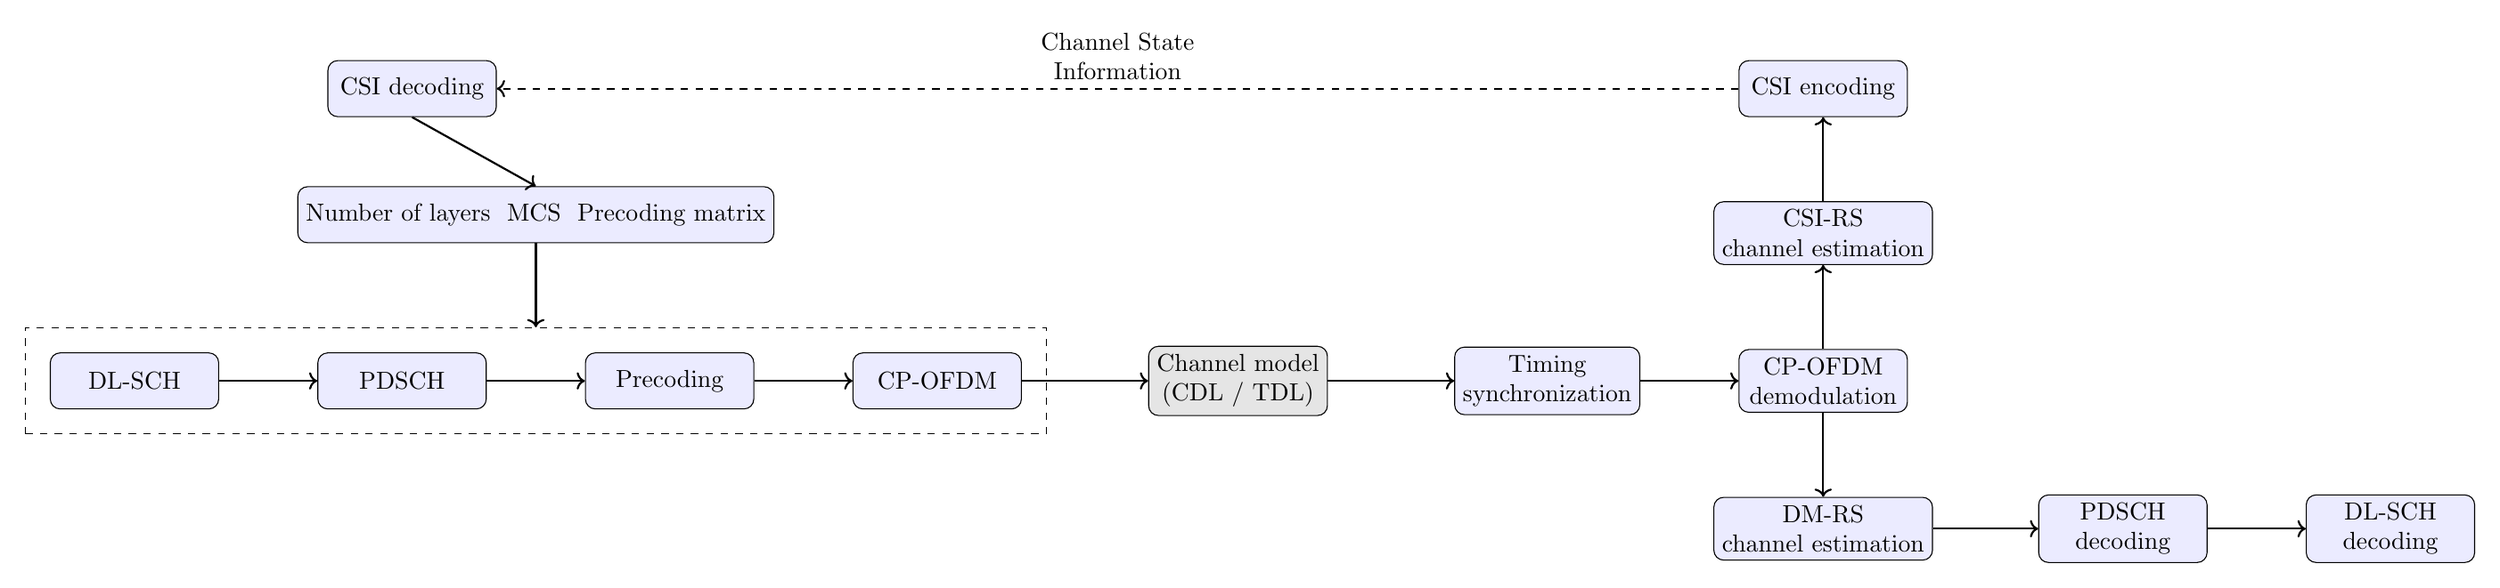
\begin{tikzpicture}[
	block/.style={
		draw,
		rounded corners,
		fill=blue!8,
		minimum height=0.8cm,
		minimum width=2.4cm,
		align=center
	},
	csiblock/.style={
		draw,
		rounded corners,
		fill=blue!8,
		minimum height=0.8cm,
		minimum width=2.4cm,
		align=center
	},
	channelblock/.style={
		draw,
		rounded corners,
		fill=gray!20,
		minimum height=0.8cm,
		minimum width=2.4cm,
		align=center
	},
	arrow/.style={->, thick},
	dashedbox/.style={draw, dashed, inner sep=10pt}
	]
	
	% ======================
	% Transmitter chain
	% ======================
	\node (dlsch) [block] {DL-SCH};
	\node (pdsch) [block, right=1.4cm of dlsch] {PDSCH};
	\node (precoding) [block, right=1.4cm of pdsch] {Precoding};
	\node (cpofdm) [block, right=1.4cm of precoding] {CP-OFDM};
	
	\draw[arrow] (dlsch) -- (pdsch);
	\draw[arrow] (pdsch) -- (precoding);
	\draw[arrow] (precoding) -- (cpofdm);
	
	% TX dashed box
	\node[dashedbox, fit=(dlsch)(pdsch)(precoding)(cpofdm)] (txbox) {};
	
	% ======================
	% Channel
	% ======================
	\node (channel) [channelblock, right=1.8cm of cpofdm] {Channel model\\(CDL / TDL)};
	\draw[arrow] (cpofdm) -- (channel);
	
	% ======================
	% Receiver chain
	% ======================
	\node (timing) [block, right=1.8cm of channel] {Timing\\synchronization};
	\node (demod) [block, right=1.4cm of timing] {CP-OFDM\\demodulation};
	
	\draw[arrow] (channel) -- (timing);
	\draw[arrow] (timing) -- (demod);
	
	% Channel estimation
	\node (csirs) [csiblock, above=1.2cm of demod] {CSI-RS\\channel estimation};
	\node (dmrs)  [csiblock, below=1.2cm of demod] {DM-RS\\channel estimation};
	
	\draw[arrow] (demod) -- (csirs);
	\draw[arrow] (demod) -- (dmrs);
	
	% Decoding chain
	\node (pdschdec) [block, right=1.5cm of dmrs] {PDSCH\\decoding};
	\node (dlschdec) [block, right=1.4cm of pdschdec] {DL-SCH\\decoding};
	
	\draw[arrow] (dmrs) -- (pdschdec);
	\draw[arrow] (pdschdec) -- (dlschdec);
	
	% CSI feedback
% === CSI encoding / decoding ===
\node (csienc) [csiblock, above=1.2cm of csirs] {CSI encoding};
\node (csidec) [csiblock, left=17.7cm of csienc] {CSI decoding};

\draw[arrow] (csirs) -- (csienc);
\draw[dashed, thick, ->] 
(csienc.west) 
to[out=180,in=0]
node[midway, above, align=center] {Channel State\\Information}
(csidec.east);

% === Control decision block ===
\node (ctrl) [block, above=1.2cm of txbox, align=center]
{Number of layers \ MCS \ Precoding matrix};

% CSI decoding -> control
\draw[arrow] (csidec.south) -- (ctrl.north);

% Control -> TX processing (whole block)
\draw[arrow] (ctrl.south) -- (txbox.north);

	
\end{tikzpicture}

	
\end{document}
